% !TEX TS-program = xelatex
% !TEX encoding = UTF-8 Unicode
% !Mode:: "TeX:UTF-8"

\documentclass{resume}
\usepackage{zh_CN-Adobefonts_external} % Simplified Chinese Support using external fonts (./fonts/zh_CN-Adobe/)
%\usepackage{zh_CN-Adobefonts_internal} % Simplified Chinese Support using system fonts
\usepackage{linespacing_fix} % disable extra space before next section
\usepackage{graphicx}
\usepackage{tabu}
\usepackage{multirow}

\begin{document}
\pagenumbering{gobble} % suppress displaying page number

\large{
  \begin{tabu}{ c l }
   \multirow{5}{1in}{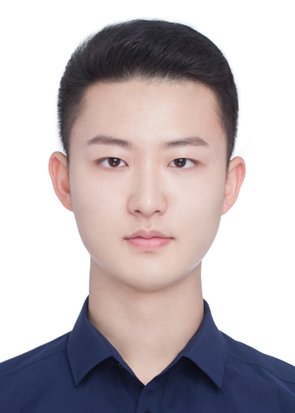
\includegraphics[width=0.88in]{avatar-1}} & \\ & \scshape \LARGE {\, 孙东旭}  \\
    & \quad \email{371211947@qq.com}  \\
    & \quad \phone{(+86) 189-7308-9012}  \\
    & \quad \github{https://github.com/sundongxu} \\
    & \quad 
\includegraphics[scale=0.02]{blog.pdf}{\ http://dongdongdong.me}
  \end{tabu}
  \\ \\

\section{\faGraduationCap\  教育背景}
\datedsubsection{\textbf{南京大学}}{2016 - 至今}
\normalsize
\textit{在读硕士} \quad 计算机科学技术系 \quad 分布式计算
\datedsubsection{\textbf{大连理工大学}}{2012 - 2016}
\normalsize
\textit{学士} \quad 国家示范性软件学院 \quad 软件工程

\section{\faUsers\ 实习/项目经历}

\datedsubsection{\textbf{腾讯} \quad OMG \quad 视频产品技术部 \quad 速看中心}{2018.07 -- 2018.09}
\normalsize
\role{实习}{后台开发}

\datedsubsection{\textbf{腾讯} \quad MIG \quad 应用宝 \quad 游戏产品中心}{2015.08 -- 2016.02}
\normalsize
\role{实习}{移动客户端开发}
\begin{itemize}
  \item 参与并完成福利中心Native导航改版、游戏页NPC弹窗、新版智能卡片、游戏内icon及预约弹框优化等多项需求,后经灰度、测试均已发布上线
  \item 2015年末代表MIG参与并主演公司年会(圣诞晚会)节目《白毛女》
  \item 作为主力先后代表应用宝与MIG参加BG内部及公司BG篮球联赛,分获亚军、季军
\end{itemize}

\datedsubsection{\textbf{SDN网络测量系统}}{2018.03 - 2018.10}
\normalsize
\role{C++/Python}{科研项目}
基于SDN仿真网络环境Mininet的网络故障分析系统(前端+后端)
\begin{itemize}
  \item 系统功能:支持网络数据包生成、路由、过滤、组装、压缩、存储、匹配
  \item 技术细节:OpenFlow协议、多线程并发同步、I/O多路复用、拓扑排序、数据库读写、正则匹配等
  \item 核心框架:消息中间件ZMQ、事件驱动库Twisted、SDN控制器Ryu、网络数据包捕获库libpcap
\end{itemize}

\datedsubsection{\textbf{RDMA网络中间件}}{2017.03 - 2017.10}
\normalsize
\role{C++/C}{科研项目,与组员合作开发}
提供类Socket接口的RDMA高性能网络框架
\begin{itemize}
  \item 系统功能:支持上层应用使用RDMA替换TCP/IP协议栈完成网络操作(消息语义、内存语义)
  \item 技术细节:TCP/IP与RDMA协议栈、多线程并发同步、内存管理、I/O多路复用、连接复用等
  \item 在Memcached、GRPC等开源项目中测试通过,延迟、吞吐量及可并发连接数量均有明显提升
\end{itemize}

\section{\faCogs\ 技术栈}
% increase linespacing [parsep=0.5ex]
\begin{itemize}[parsep=0.5ex]
  \item 语言: C++/C > Java == Python
  \item 平台: Linux/MacOS
  \item 自评:
      理解面向对象思想,熟悉基本数据结构及常用算法,并熟练掌握C++及GCC、GDB及Vim等开发工具的使用;
      多次C++/Java/Android项目经历,并能利用Python进行数据分析;
      长期工作在Linux系统环境下,熟悉常用命令与服务器操作,并具有较为扎实的网络编程理论基础,了解基本Shell脚本编程;
      热爱钻研,对操作系统内核机制兴趣浓厚
\end{itemize}

\end{document}
